\documentclass[nofilelist]{cslthse-msc}
% to show a list of used packages at the end of the document, delete the nofilelist option
%\documentclass{cslthse-msc}
\usepackage[utf8]{inputenc}
\usepackage[english]{babel}
\usepackage{amsmath}
\usepackage{amsthm}
\usepackage{graphicx}
\usepackage[titletoc, header, page]{appendix}
\usepackage{transparent}
\usepackage{xcolor}
\usepackage[
	backend=biber,
	style=numeric,
	sorting=none,
]{biblatex}
\addbibresource{report.bib}
\usepackage{parskip}

% used to display the used files at the end. Select nofilelist as a package option to disable this
%\listfiles % initialize

%\geometry{showframe}
%better like this?
%\student{Flavius Gruian}{Flavius.Gruian@cs.lth.se}
\student{Stefan Eng}{atn08sen@lu.se}

\thesisnumber{LU-CS-EX: 2020-XX} % Birger Swahn will provide this number to you, once the thesis is ready for publication

\title{
  Usability testing on the web; Measuring how design impacts task performance
  times.
}

%\onelinetitle
%\twolinestitle
\threelinestitle
%\fourlinestitle

%\subtitle{A {\LaTeX} class}
\company{MASSIVE}
\supervisors{
  John Deer, \href{mailto:jdeer@company.com}{\texttt{jdeer@company.com}}
}{
  Don Jeer, \href{mailto:djeer@xy.lth.se}{\texttt{djeer@xy.lth.se}}
}
\examiner{Jane Doe, \href{mailto:jane.doe@cs.lth.se}{\texttt{jane.doe@cs.lth.se}}}

\date{\today}
%\date{January 16, 2015}

\acknowledgements{
}

\theabstract{
}

\keywords{
	Usability testing,
	Web-application,
	Flask,
	HTML
}

\begin{document}
\renewcommand{\bibname}{References}

\makefrontmatter
\newcommand{\todo}[1]{\textcolor{blue}{\textbf{TODO:} #1}}
\newcommand{\eatdot}[1]{}
\newcommand{\ctitle}[1]{\citetitle{#1}\cite{#1}}
\newcommand{\vv}[1]{\input{vars/#1.txt}\unskip}

\chapter{Introduction}

	Usability is traditionally done in person with the
	\textit{over the shoulder} method which gives a good insight of what a
	participant does during a test. Further more, if the
	\textit{thinking out aloud - method} is utilized correctly, the
	test-moderator should have a good insight into the participant
	thought-process during the test.

	\todo{Expand usability-testing introduction.}

	While effective[?] this method scales poorly with a one to one ratio between
	moderator and test participant. This project investigates the possibility of
	alleviating this scale-constraint by using a internet-based platform for
	usability-testing home-grown user interface.

	\section{Usability testing, then and now}

		\todo{Expand this section.}

	\section{Report goals}

		\begin{enumerate}
			\item{Create a web based platform for usability testing.}
			\item{Run one or several interface tests with real users on the platform.}
			\item{
				Verify that the collected data shows a significant[?] impact on the studied
				variable(s) when parameters are changed. \todo{Shorten?}
			}
		\end{enumerate}

	\section{Literary scope}

		This report draws and builds on information from the fields of usability
		testing, web design and interaction design.

		Specifically, \ctitle{cite_handbook_usability} and
		\ctitle{cite_usability_testing_essentials}, provide a contrast between
		traditional and modern approaches to usability testing and how to perform
		them.

		\ctitle{cite_don_make_me_think} provides a concise and interesting
		summary of no-nonsense approaches to web design from a usability perspective.
		Last but not least \ctitle{cite_the_design_of_everyday_things} introduces
		both \textit{user-centered-} and \textit{interaction-design} together
		with the concept of \textit{affordances},

	  %Introduction to user interface design and usability testing? \\
	  %
		%Figure out how much of an impact different design aspects have on tasks
		%that require distinguishing one element from another. And doing it in a
		%decentralised manner based on web-application. \\
	  %
	  %Don't make me think -> webdesign. \\
	  %Design of everyday things -> webdesign. \\
	  %Report based on distances / colors -> webdesign. \\
	  %Usability-testing guide -> webapp suggesting + other. \\


	\chapter{Approach}

		\section{Method}

			Results by measuring the time and showing graphs + statistical grouping /
			analyzis.

			\subsection{Threats to validity}

				network latency?
				multiple runs with same person?


		\section{Theory}

			The theory contains color-theory and the experience from managerial
			positions.

			\subsection{Information and color}

			\subsection{Measuring completion times}

			\subsection{Representative tasks}

		\section{Implementation}

			Writing a web-application with Flask + python + sqlite3.
			HTML5 and CSS with a dab javascript.

			\subsection{Platform software stack}

			\subsection{Interface creation}

			\subsection{Variable challenges}

	\chapter{Evaluation}

		\section{Results}

			\subsection{Participation, tests and ratio correct answers}

				The test-site went live 2020-01-24 and the link was mainly shared on
				Facebook in the following days. 2020-01-27 the link was shared on
				the MASSIVE internal mailing list, boosting the participation
				significantly, resulting in a total of
				\vv{total_participants} participants.

				\begin{figure}[h!]
					\centering
					\includegraphics{figures/participants_over_time.pdf}
					\caption{Total registered participants over time.}
				\end{figure}

				In total \vv{total_tests} tests were run, where
				\vv{total_tests_correct} were answered correctly,
				\vv{total_tests_uncompleted} never produced an answer, leaving
				\vv{total_tests_incorrect} incorrect answers.

				\begin{figure}[h!]
					\centering
					\includegraphics{figures/runs_over_time.pdf}
					\caption{Total test-runs over time with number of correct answer.}
				\end{figure}

		\section{Discussion}

			\subsection{Possible Improvements}

	\chapter{Conclusions}

		Did it have an significant impact? Was the web the correct platform? What
		could be done better over the internet? Recording screen and voice?
		(Javascript, since it's already used, pull up some statistics?)

	% Should use consistent formatting when it comes to Names ("FirstName LastName", or "F. LastName")
	\makebibliography{report}

	%make sure we're on even page with the pop-sci
	\checkoddpage
	\ifoddpage
	\else
		 \newpage
		 \thispagestyle{empty}
		 \mbox{ }
	\fi
	%\begin{appendices}
	%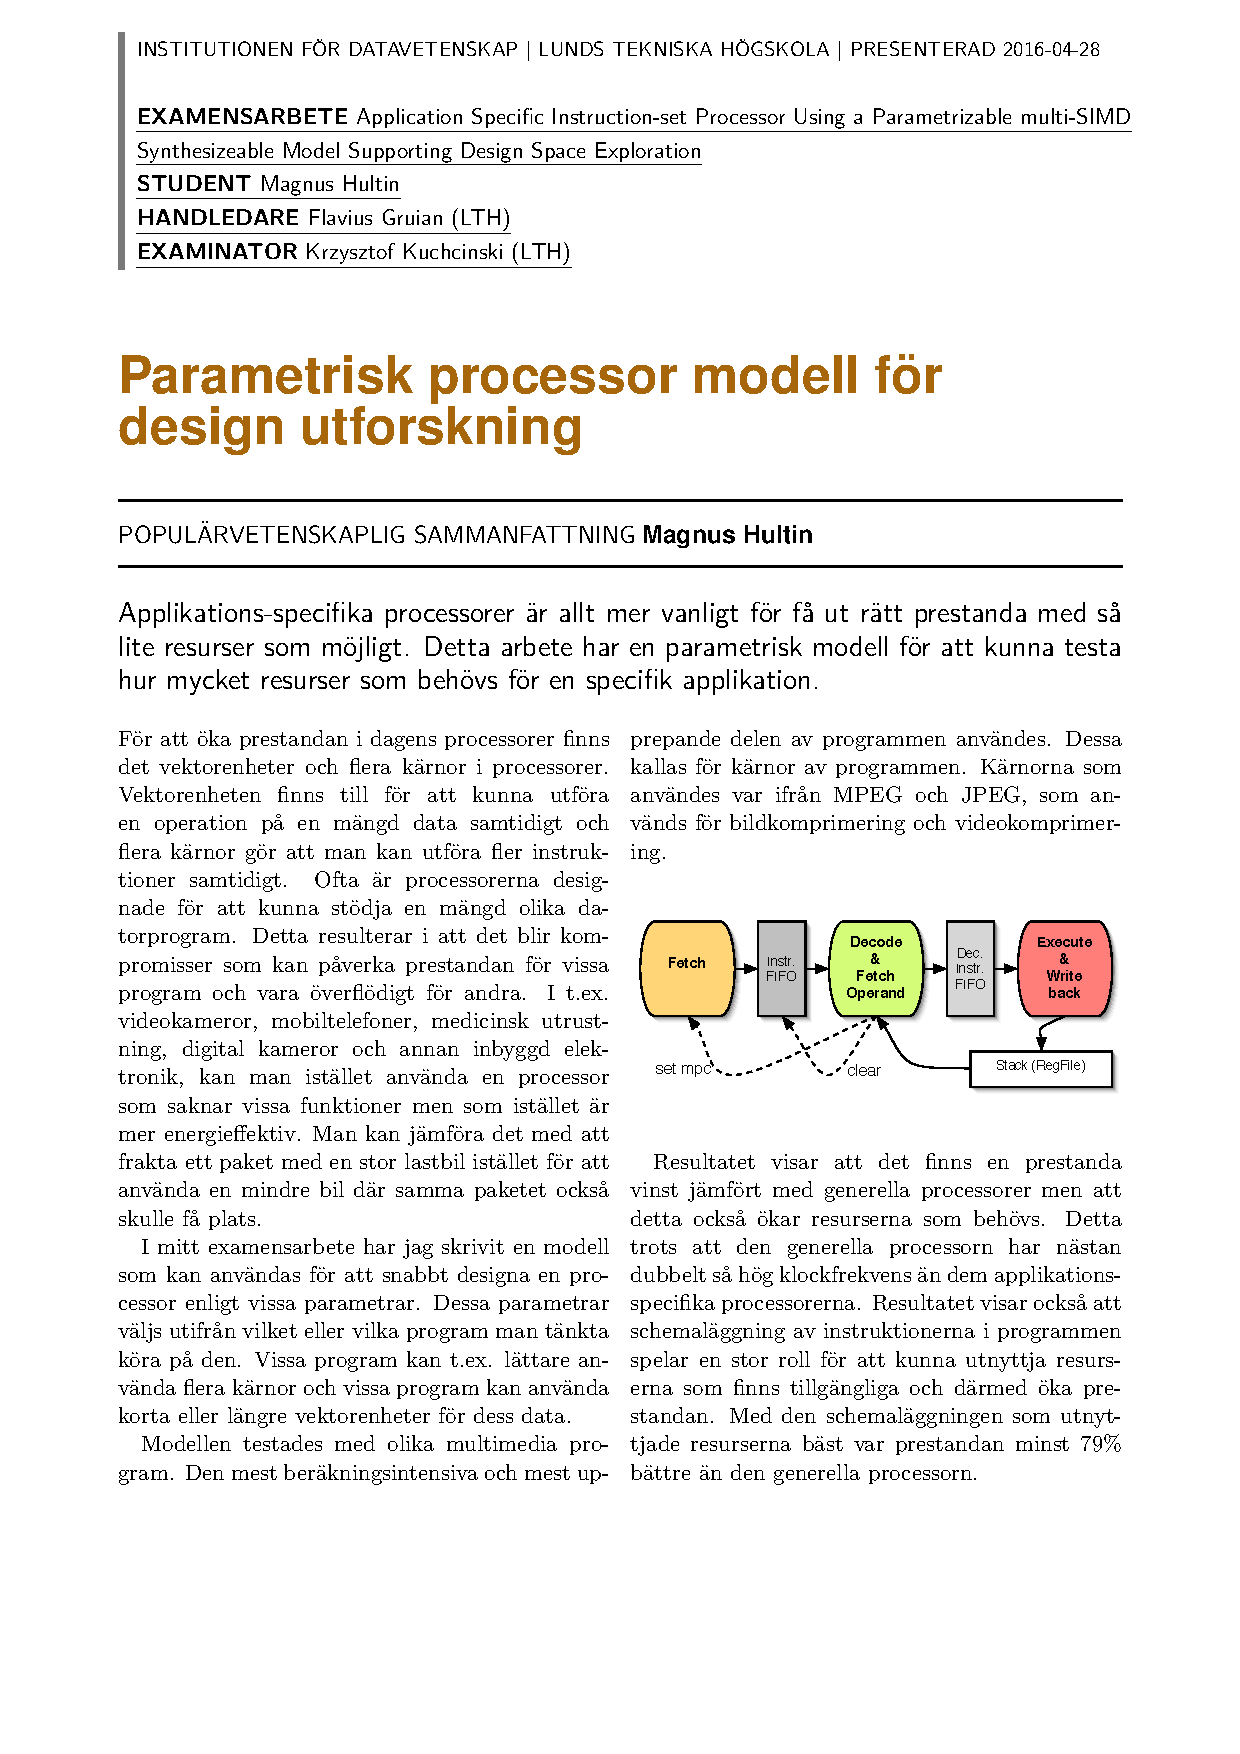
\includepdf[pages={1}]{popsci/popsci.pdf}
	%\end{appendices}

\end{document}
